\documentclass[sigconf,authorversion,nonacm, 11pt]{acmart}

\usepackage{blindtext}
\usepackage{multicol}
\usepackage{array}
\usepackage{caption}
\usepackage{wrapfig}
\usepackage{listings}
\usepackage{caption}
\usepackage{subcaption}
\usepackage{acronym}
\usepackage{amsmath}
\usepackage{cleveref}
\usepackage{mathtools}
\usepackage{makecell}
\usepackage{booktabs} 
\usepackage{balance}
\usepackage{xspace}
\usepackage{balance}
\usepackage{circledsteps}
\usepackage{textcomp}
\usepackage{amsmath,amssymb,amsfonts}
\usepackage{graphicx}
\usepackage{textcomp}
\usepackage{xcolor}
\usepackage{multirow}
\usepackage{algpseudocode}
\usepackage{algorithm}

\acrodef{fsm}[FSM]{Finite State Machine}
\acrodef{dsa}[DSA]{Domain-Specific Architecture}
\acrodef{rei}[REI]{Regular Expression Inference}
\acrodef{ml}[ML]{Machine Learning}
\acrodef{ssa}[SSA]{Static Single-Assignment}
\acrodef{re}[RE]{Regular Expression}
\acrodef{nlp}[NLP]{Natural Language Processing}
\acrodef{ast}[AST]{Abstract Syntax Tree}
\acrodef{eda}[EDA]{Electronic Design Automation}
\acrodef{itp}[ITP]{Interactive Theorem Proving}
\acrodef{cegar}[CEGAR]{Counterexample-Guided Abstraction Refinement}


\acrodef{gpu}[GPU]{Graphic Processing Unit}
\acrodef{fpga}[FPGA]{Field Programmable Gate Array}
\acrodef{rtl}[RTL]{Register Transfer Level}
\acrodef{ir}[IR]{Intermediate Representation}

\begin{document}

\title{Democratizing Hardware Verification By Formalizing High-Level Abstractions}

\author{Luisa Cicolini}

\maketitle
\thispagestyle{empty}

\textit{
    Verification is a fundamental step of the hardware design process, preventing expensive and potentially critical mistakes.
    As the complexity of hardware designs increases, so does the need for more efficient verification strategies to streamline the overall process.
    The CIRCT \ac{eda} stack has recently shown that explicit representations of higher-level, domain-specific hardware enable the effective generation of optimized Verilog code.
    Such higher-level hardware representations can be a game changer in verifying the designs progressively as they are lowered and exploring novel, domain-specific verification approaches. 
    However, taking advantage of these representations for verification purposes remains challenging due to the lack of formalized semantics for high-level abstractions, which often rely on domain-specific structures such as \acp{fsm}.
    In my PhD I will exploit modern multi-level EDA approaches to formally verify the semantics of high-level, domain-specific hardware abstractions, making the manipulation and verification of their semantics scalable and white-box.
    In particular, I aim to
    (1) formalize higher-level abstractions to guide lower-level verification efforts, 
    (2) verify transformations from several high-level level abstractions to low-level ones (e.g. in the CIRCT ecosystem), and
    (3) explore domain-specific decision procedures and reasoning frameworks for verifying higher-level abstractions, such that the verification evolves as the design is lowered. 
    This work will make hardware verification accessible in the early stages of the design process in a white-box framework that can take advantage of different domain-specific abstractions and design paradigms.
}   


\section{Introduction}

\begin{figure*}[ht]
    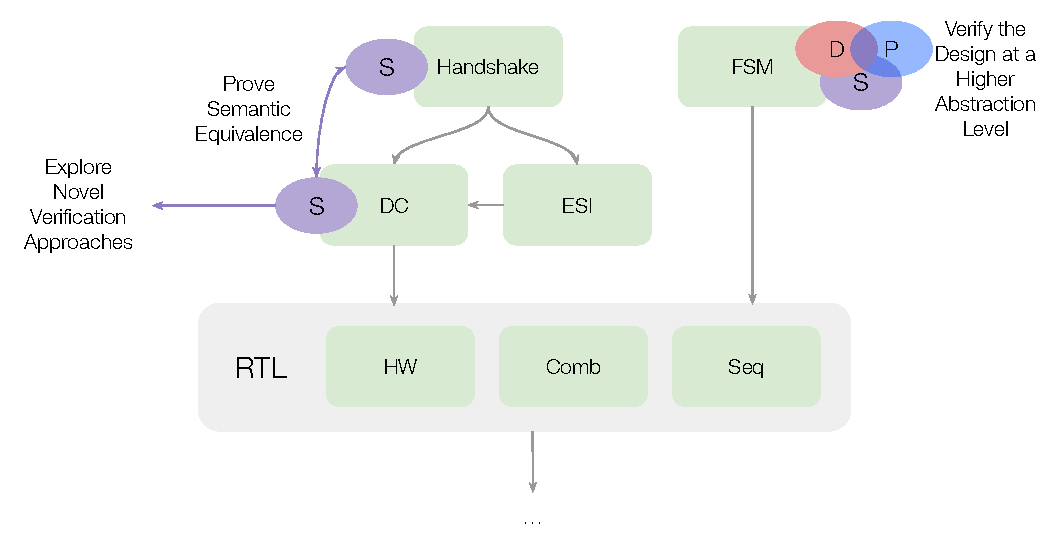
\includegraphics[scale=0.8]{semantics.pdf}
    \caption{Formalizing the semantics (S) of CIRCT dialects in Lean4 will allow us to (1) verify the compilation and equivalence 
    between different abstractions, (2) explore novel verification approaches in a verified environment, (3) verify whether a property
    (P) holds for a design (D) at a certain level.}
\end{figure*}

Designing modern hardware is incredibly complex, even more so as the demand for domain-specific architectures increases to compensate for the decline of general-purpose ones~\cite{asanovic2006landscape, hennessy2018new}. 
Verification plays a crucial role in the process, as it can uncover expensive and potentially critical mistakes before the tape-out: yet, it also represents a bottleneck for the design procedure~\cite{foster2013design, wilson2020verifstudy, vasudevan2021learning}. 
To address these challenges, the CIRCT project~\cite{circt, mlir_circt} introduces a novel concept of hardware compiler that supports different frontends and backends and comprises various domain-specific abstractions (\textit{dialects}), making the compilation of a design progressive, through different lowerings and dialects. 
Thanks to tailored domain-specific abstractions, CIRCT allows designers to use local reasoning to analyze and optimize the numerous domain-specific concepts it models.
For example, in CIRCT~\cite{circt, mlir_circt}, high-level abstractions such as \acp{fsm} or latency-insensitive \acp{ir} are optimized and progressively lowered to \ac{rtl} and Verilog, generating production-quality, optimized code~\cite{circt_sifive}. 
Besides making hardware design more flexible, the high-level abstractions CIRCT exposes also have great potential for verification.
Exploiting higher-level abstractions to bring verification tasks to a higher level and guide lower-level verification tooling already proved a successful approach~\cite{huang2018instruction, chen2021leveraging, mattarei2018cosa, hunt2006sat}.
CIRCT represents an excellent infrastructure to expand and make the most of this approach, given the domain-specific abstractions it includes.

Overall, \textbf{bridging domain-specific abstractions and verification tooling} is a fundamental step to make sure that verification is up-to-speed with the recent domain-specific hardware design trends, and CIRCT is the perfect environment to validate this approach, thanks to the numerous abstractions it provides. 
However, taking advantage of high-level CIRCT \acp{ir} remains a complex task due to the lack of precise semantics and documentation. 
In particular, the most critical challenges involved in the formal verification of the semantics of such diverse dialects and domain-specific abstractions are 
(1) precisely defining the semantics of the dialects relying on little-to-no documentation, 
(2) identifying and using effective automatic reasoning tools for the formalization, 
(3) managing the semantics evolution during the lowering through different abstractions. 

With this work, I intend to tackle these challenges, combining my experience with CIRCT and with the Lean4 \ac{itp} to expose the semantics of high-level abstractions and improve the scalability and accessibility of verification. 

\section{Related Work}

Previous works tackled the formalization and definition of semantics in hardware description languages, considering different levels of abstraction~\cite{melham1988abstraction}. 
Managing the different design paradigms on which domain-specific abstractions rely is incredibly challenging in this context. 
Promising efforts also exist bridging hardware compilers, and CIRCT specifically, with formal methods. 
However, these are currently limited in exploiting high-level abstractions due to the complexity and low flexibility of the verification tools they rely on, for example, SAT and SMT solvers.
Lean4 is currently the best option for reasoning about the semantics of CIRCT-like infrastructures, as proven by the Lean-MLIR~\cite{bhat2024verifying} framework, as it provides a flexible and verified environment to encode and manipulate domain-specific dialects.

Koika~\cite{bourgeat2020essence} directly derives from Bluespec~\cite{bluespec} and features novel and deterministic operational semantics, including a verified compiler to circuits. 
In particular, Koika focuses on the importance of cycle-accurate description (and semantics) when dealing with the performance of circuits without compromising on the straightforward description of their functional properties. 
The authors also highlight how traditional HDLs and HLS compilers lack precise semantics, making describing complex interactions between different modules difficult.

ReWire~\cite{procter2015semantics} introduces a functional programming language with a compiler that translates the high-level description of a design into working hardware relying on the language's semantics to describe its behaviour.

Chisel~\cite{bachrach2012chisel} is another powerful structural language embedded in Scala, also used as a frontend for CIRCT. 

Bernstein et al. ~\cite{bernstein2021semantics} propose a description of hardware semantics at different abstraction levels within an abstract interpretation framework, mainly focusing on the representations used in the early phase of the design when reasoning at the latency-insensitive level of the hardware representation.

Another work exploits ACL2~\cite{hunt2006sat} to encode the semantics of \acp{fsm} for the verification of hardware designs, extracting said \acp{fsm} from lower-level representations.
This work is deeply inspiring for my PhD since CIRCT naturally exposes the \ac{fsm} representation of its designs.

Managing the evolution of domain-specific semantics where different abstractions meet, e.g. latency-insensitive and cycle-accurate ones, is a core challenge of my work.
In particular, the semantics of latency-insensitive abstractions and their relationship to cycle-based representations are incredibly challenging. 
In this context, Carloni et al. ~\cite{carloni2001theory} introduce a theory to describe and represent latency-insensitive circuits and systems. 
The idea is to represent complex systems considering their single functional components and communication according to a specific protocol. 
The theory introduced allows for the composition of such single components into a complex system to satisfy synchronization and communication properties. 

Due to the numerous abstractions CIRCT exposes, its correctness guarantees require careful reflection on the semantics of the various \acp{ir} involved and the lowerings between them. 
A first recent work~\cite{zhao2024k} provided a preliminary formalization of CIRCT dialects, only focusing on lower-level \acp{ir}. 

Within CIRCT, \texttt{circt-lec} and \texttt{circt-bmc} are other tools that perform logical equivalence checking and bounded model checking, respectively, at the \ac{rtl} level. 
CIRCT also features different lowerings to standard hardware verification formats, such as \texttt{btor2}~\cite{btor2, niemetz2018btor2}, \texttt{aig}~\cite{aiger2} and \texttt{SMT-LIB}~\cite{barrett2010smt}, that contribute to integrating verification within the hardware design process.

Moreover, the SMT dialect represents one means of formalizing dialects' semantics at different levels. 
This dialect comprises most SMT-LIB~\cite{barrett2010smt} operators. 
It is the endpoint of various lowerings from different dialects, meaning that their semantics are encoded in SMT-LIB for verification purposes.
The dialect is part of the compiler verification and optimization efforts currently under development in a research group at the University of Cambridge, with whom I have worked for the past year. 
However, the underlying complexity of SMT solvers such as z3~\cite{de2008z3} and their low flexibility make it hard to embed such domain-specific information into the actual SMT model. 
Lean4 can tame this complexity: it is an open-source programming language and theorem prover providing a flexible environment to write verified code. 

Works such as Lean-MLIR~\cite{bhat2024verifying} have already proved the benefits of embedding MLIR~\cite{mlir} dialects' semantics in Lean4.
This framework can also be game-changing in expanding CIRCT verification tooling.
Lean4 enables writing theorems that encode certain domain-specific behaviours and successfully guide the verification with significantly higher trust than standard verification tooling.
We typically need to trust SMT and SAT solvers when verifying a design. 
For instance, consider z3~\cite{de2008z3}: it consists of a vast C++ codebase, it is not verified, and these characteristics make extending its tactics and logic incredibly hard, as shown, for example, by previous efforts to expand it for \acp{chc} reasoning~\cite{gurfinkel2022program}. 
As a consequence, optimizing the job of the SMT solver, for example, by introducing tactics that exploit domain-specific knowledge available at higher abstraction levels, is not a practically viable solution. 
On the contrary, Lean4 has already proved very effective in building white-box automation techniques for bitvector manipulation (to which I contributed) and verification. 
In particular, the \texttt{bv\_decide} tactic~\cite{bvdecide} represents a first effort in this space, implementing a verified bit-blaster and LRAT checker.
This fact demonstrates the potential of Lean4 in the verification field and the community's interest in working towards this direction. 
Moreover, thanks to its flexibility, Lean4 represents the perfect environment to experiment with further verified verification methods such as abstract interpretation.

\section{Research Direction and Challenges}

\begin{figure*}[ht]
    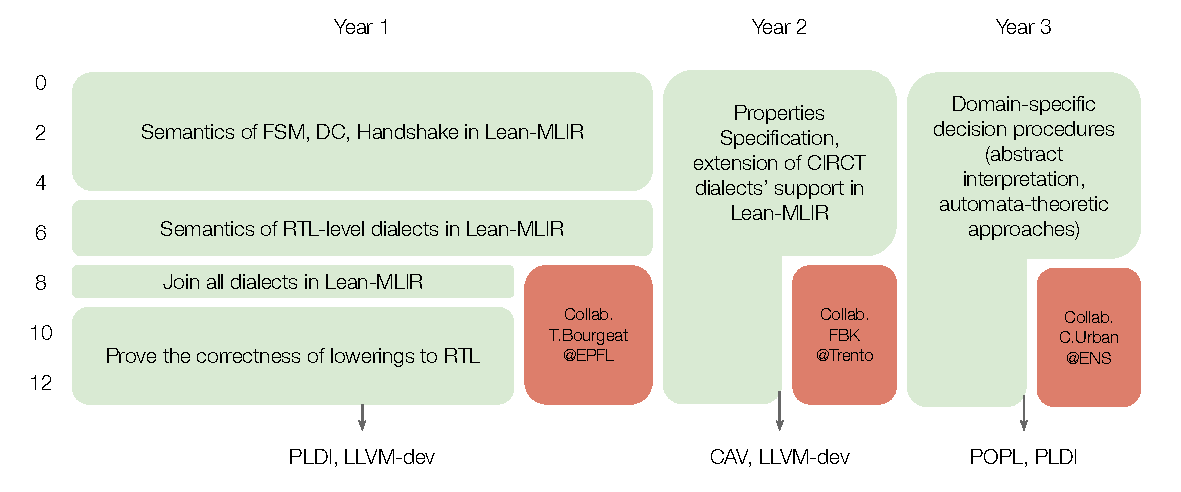
\includegraphics[scale=0.8]{logistics.pdf}
    \caption{
        I will spend the first four months of the PhD implementing in Lean4 the semantics of three high-level dialects (FSM, Handshake, DC) and studying the state-of-the-art works concerning the semantics of these domain-specific representations.
        Then, I plan to spend three more months implementing the semantics of the CIRCT dialects necessary for the RTL-level representation (Hardware, Comb, Seq). 
        During the following month, I will work on combining these dialects in the Lean-MLIR framework to ensure the correctness of the overall semantics and their flexibility and functionality. 
        During the last four months of the first year, I will prove the correctness of the lowerings from the higher-level abstractions to RTL, collaborating with Thomas Bourgeat's research group at EPFL. 
        The second year will focus on implementing the property specifications in Lean-MLIR. I also aim to visit Fondazione Bruno Kessler (FBK) and the University of Trento. 
        I will investigate alternative decision procedures and verification frameworks for domain-specific representations during the last year, collaborating with Caterina Urban's research group at ENS. PLDI, POPL, and CAV are the leading conferences I intend to target, in addition to LLVM developer meetings. 
    }
    \label{fig:logistics}
\end{figure*}

During my PhD, I aim to enhance verification efforts for the CIRCT infrastructure by formally verifying the semantics of its dialects to enable the verification of lowerings and optimizations, the progressive verification of designs' properties, and the adoption of novel verification techniques. 
Following the path indicated by Lean-MLIR~\cite{bhat2024verifying}, I intend to formalize more high-level abstractions and dialects, starting from the \ac{fsm} dialect and also considering those relying on radically different design paradigms from traditional imperative or functional \acp{ir}, such as the Dynamic Control (DC) dialect. 
This aspect will require careful mathematical modelling of complex, dataflow-like behaviour to fill gaps in the informal model, e.g. where latency-insensitive and circuit-based semantics meet. 
Besides introducing a powerful means to reason about dialects' semantics and the overall correctness of the compilation and the designs, this work will also lay the foundations for including higher-level verification techniques into CIRCT, for example, those leveraging automata-theoretic and abstract-interpretation-based approaches. 

This work combines CIRCT's high-level information at different abstraction levels with Lean4's flexibility and minimal trusted codebase. 
Until now, verifying high-level abstractions with standard lower-level hardware verification techniques (such as assertion-based verification or SMT solvers) has been very complex ~\cite{symbiyosys, witharana2022survey}, due to the scarce flexibility of the tools involved (e.g. z3~\cite{de2008z3}) and the limited number of abstractions they support. 
With this work, I aim to formalize the high-level information CIRCT exposes to bring verification to a higher level and possibly guide the effort of lower-level, classical verification approaches, relying on the flexibility of Lean4.
The formalization of dialects within Lean4 also enables the verification of compiler passes, offering further guarantees for the correctness of CIRCT itself. 

Lean4 is a fertile, open-source environment to work on verification frameworks thanks to its flexibility, versatility, and trust level. 
Moreover, working in an open-source environment is an incredibly valuable aspect of this work, as it significantly increases the quality of the output - thanks to peer-review processes - and creates impact, being available to numerous users.  

Moreover, formalizing the semantics of CIRCT dialects allows semantics manipulation up to a point where the application of different verification approaches is possible and beneficial. 
Exploring different approaches in the context of hardware verification is currently a challenge~\cite{mukherjee2015hardware, malik2008hardware}, requiring significant effort to bridge the hardware level with a suitable abstraction that alternative verification methodologies, such as abstract interpretation frameworks, can digest. 
Nevertheless, preliminary studies suggested the effectiveness of these methodologies, especially at specific abstraction levels~\cite{bernstein2021semantics}. 
Formalizing the semantics of CIRCT dialects in an interactive theorem prover is a game-changer in this context, as it proves a stable foundation to explore many verification strategies.

Overall, formalizing the semantics of a large subset of CIRCT's dialects is a first step towards integrating the \ac{eda} toolchain with automatic verification, which is simultaneous and progressive with the design procedure and comprises different verification techniques. 
While this aspect can increase the compilation time for a single design iteration, its correctness guarantees can significantly reduce the number of iterations required to generate the desired design, eventually improving the overall design pipeline.
Moreover, this work paves the way for filling and reasoning about subtle semantics gaps in hardware abstractions, by introducing formally verified semantics in the CIRCT ecosystem.

\section{Research Organization}

Figure~\ref{fig:logistics} summarizes the organization of my PhD.
This research proposal comprises three milestones, which I plan to distribute in the three years of the PhD: 
\begin{enumerate}
    \item The goal of the first year is to \textbf{formalize the semantics of a first subset of high-level CIRCT dialects} (namely FSM, Handshake and DC) and \textbf{verify their lowering to RTL level within Lean-MLIR}.
    This phase will require careful study of existing works, especially concerning the formalization of latency-insensitive behaviours in DC and their interface with cycle-accurate representation. 
    Then, I will implement the semantics of the CIRCT dialects necessary for the RTL-level representation (Hardware, Comb, Seq) and spend some time combining all these dialects in Lean-MLIR. 
    As a final task for the first year, I will prove the correctness of the lowerings from the higher-level abstractions to RTL, including some of the optimizations involved.
    I will target PLDI to publish the formally verified semantics resulting from this work and present it at LLVM-dev meetings.
    Thomas Bourgeat and his research group, with whom I am already working, represent an excellent collaboration opportunity at this stage of the PhD because of their expertise in hardware semantics definition and verification. 
    \item \textbf{Bringing designs' verification at a higher abstraction level, exploiting different dialects and their formalized semantics}. 
    At this point, a crucial step is understanding how to correctly specify relevant properties, which will require thorough readings in the state of the art. 
    Moreover, I plan to add further dialects to the Lean-MLIR framework during the second year. 
    During the second year, I intend to collaborate with Stefano Tonetta's research group at Fondazione Bruno Kessler (FBK) due to their expertise in developing verification techniques and solvers. 
    CAV is the ideal conference to publish the output of this second year.
    \item \textbf{Explore different verification strategies}, such as automata-theoretic approaches and abstract interpretation frameworks, to fully take advantage of the formalized semantics. 
    During the last year, I plan to take advantage of the effort put into effectively formalizing CIRCT dialects. 
    I will investigate how other verification techniques can take advantage of the formalized semantics to improve the guarantees concerning the design's behaviour, aiming to reduce the number of necessary iterations. 
    To work on these topics, I intend to collaborate with Caterina Urban's research group at ENS, given the high-impact work they have carried out in abstract interpretation and semantics analysis. 
    PLDI and POPL are the conference targets for publishing the output from this last year. 
    \item I plan to spend six additional months writing the \textbf{PhD thesis}, which will focus on how CIRCT and Lean4 are a unique combination of tools to make hardware verification flexible and extensible, bending its tools to fit different designs and techniques.
\end{enumerate}
The work of the next 3.5 years is a starting point to becoming an expert in hardware verification, building valuable connections and laying the foundations for the research work to come as I continue my career in academia and pursue my dream of becoming a professor.

\thispagestyle{empty}
\bibliographystyle{acm}
\bibliography{biblio}
\thispagestyle{empty}
\end{document}
